
\section{Identification of the boat parameters} \label{sec:part1}

\subsection{Transfer function from $\delta$ to $\psi$}
To start out this assignment we want to find the transfer function from $\delta$ to $\psi$, parameterized by T and K. By assuming no disturbances ($b=0$), using \cref{eq:psidot} and \cref{eq:rdot_def}, and laplace transform with the zero initial condition we find
\begin{equation*}
    \ddot{\psi} = -\frac{1}{T}\dot{\psi} + \frac{K}{T}(\delta - b)
\end{equation*}
\begin{equation*}
    s^2\psi = -\frac{1}{T}s\psi + \frac{K}{T}\delta
\end{equation*}
\begin{equation} 
    H(s) =  \frac{\psi(s)}{\delta(s)} = \frac{K}{s(Ts+1)}
\end{equation}

\subsection{Parameters in smooth weather conditions}

We now want to identify the parameters in smooth weather conditions, with all disturbances 
With all disturbances turned off. Find T and K, with $\omega_1 = 0.005$ and $\omega_2 = 0.05$. Leser av plottene og finner A (for amplitude): $A_1 = 29.354$ og $A_2 = 0.831$. 

\begin{figure}[H]
\begin{subfigure}{0.5\textwidth}
    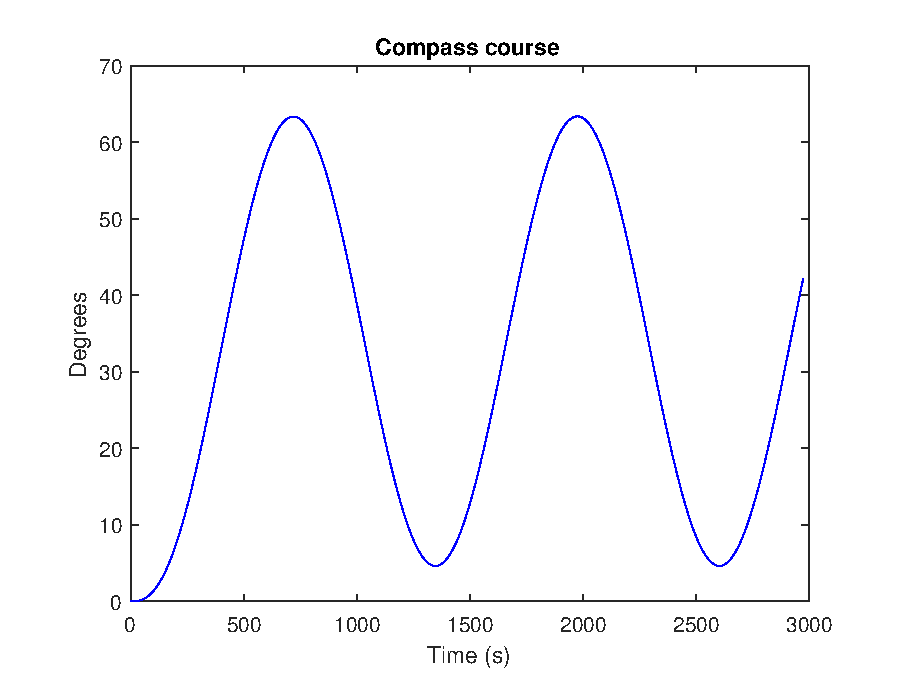
\includegraphics[width=1\linewidth]{Part1_pics/p1b_omega1.eps}
    \caption{$\omega_1$}
\end{subfigure}
\begin{subfigure}{0.5\textwidth}
    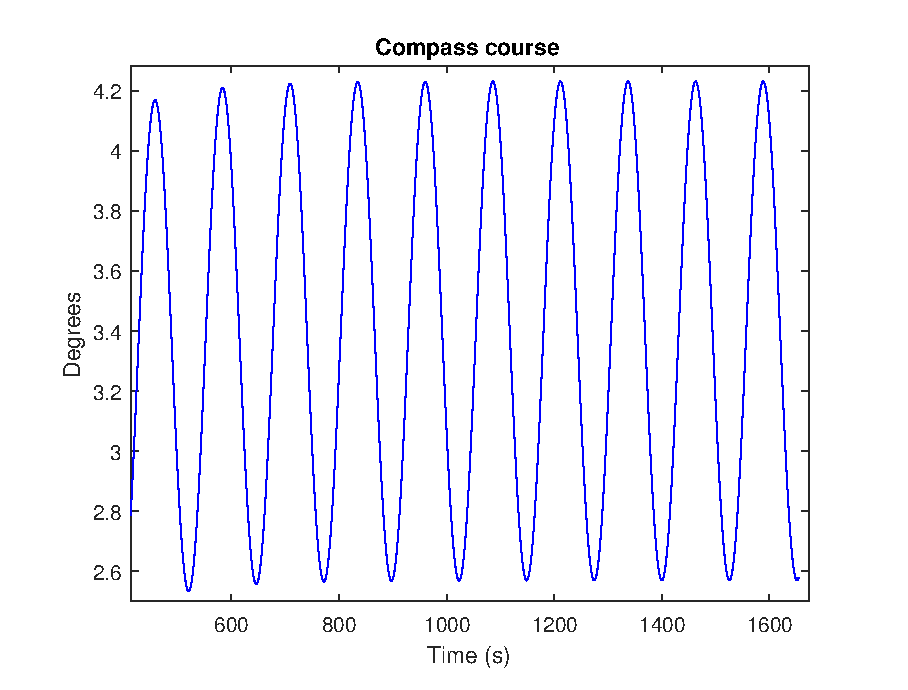
\includegraphics[width=1\linewidth]{Part1_pics/p1b_omega2_zoomedin.eps}
    \caption{$\omega_2$}
\end{subfigure}
\caption{Output of the Compass with $\omega_1$ and $\omega_2$}
\label{fig:p1b}
\end{figure}

Bruker ligningssett og finner T og K ved hjelp av 
\begin{equation} \label{eq:transferfunction}
\begin{split}
    |H(j\omega)| &= \left| \frac{K}{j\omega(Tj\omega + 1)} \right| \\
    &= \frac{K}{\omega \sqrt{T^2 \omega^2 + 1}} \\
    &= A
\end{split}
\end{equation}
where $j = \sqrt{-1}$ for $\omega_1$ and $\omega_2$. From this we find by, isolating K, an expression for T
\begin{subequations}
\begin{equation}
    K = A_1 \omega_1 \sqrt{T^2 \omega_1 + 1} = A_2 \omega_2 \sqrt{T^2 \omega_2 + 1} \label{eq:K_def}
\end{equation}
\begin{equation}
    T^2 = \frac{A_2^2 \omega_2^2 - A_1^2 \omega_1^2}{A_1^2 \omega_1^4 - A_2^2 \omega_2^4} \label{eq:T_def}
\end{equation}
\end{subequations}
By changing the constants for their numbers: $T \approx 72.4264$ and $K \approx 0.1561$.

\subsection{Parameters with waves and measurement noise}
Oppg: Repeat part b) with waves and measurement noise turned on. This corresponds to identifying the parameters in rough weatherconditions. Is it possible to get good estimates of the boat parameters in this case?
\bigskip

\textbf{pk\_omega1.eps} - - - With low pass filter we might be able to get good parameters. To do this we take the average of the peak values of the signal with noise. Take topp (topp = top/peak) punkter and bottom points with noise and calculate the amplitude. with $\omega = 0.005$: Tar og regner forskjellen mellom topp og bnn to forskjellige steder og tar snittet av dem:
\begin{equation*}
    A_{1,1} = \frac{65.34 - 2.702}{2} = 31.344
\end{equation*}
\begin{equation*}
    A_{1,2} = \frac{65.47 - 2.495}{2} = 31.4875
\end{equation*}
The average of $A_{1,1}$ and $A_{1,2}$ then becomes 31.41575. With $\omega_2 = 0.05$ the signal became very noisy and hard to read. We see that we can estimate top and bottom point.
\bigskip

\begin{figure}[H]
    \centering
    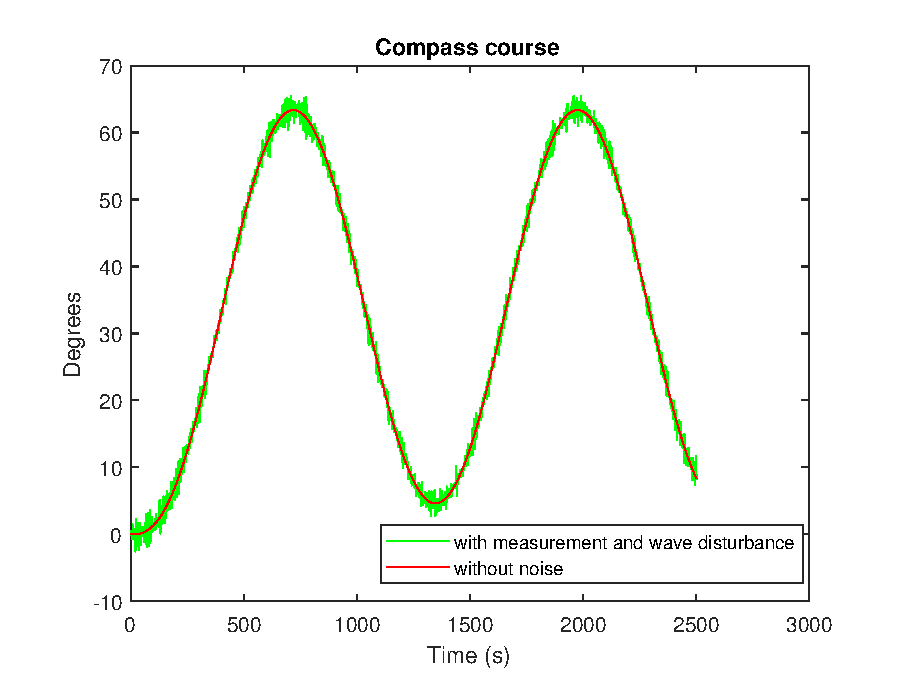
\includegraphics[width=0.5\linewidth]{Part1_pics/p1c_omega1_comp.eps}
    \caption{Compass comparison with $\omega_1$ and added noise}
    \label{fig:p1c1}
\end{figure}
\textbf{plc\_omega2\_comp.esp} - - - To find top and bottom point for the amplitude corresponding to $A_2$. Take the average of the amplitude values the same method as with $A_1$.

\begin{equation*}
    A_{1,1} = \frac{5.384 - 1.942}{2} = 1.721
\end{equation*}
\begin{equation*}
    A_{1,2} = \frac{6.36 - 1.451}{2} = 2.4545
\end{equation*}
\begin{equation*}
    A_{1,2} = \frac{6.321 - 0.2752}{2} = 3.0229
\end{equation*}
Giving the average for $A_2$ as 2.39946. To calculate the new K and T for the system with waves and noise turned on, we used MATLAB script:

...

which gave $T_c = 290.67$ and $K = 0.1576$. The new T varied quite a bit from b). No good estimate with noise. 
\begin{figure}[H]
    \centering
    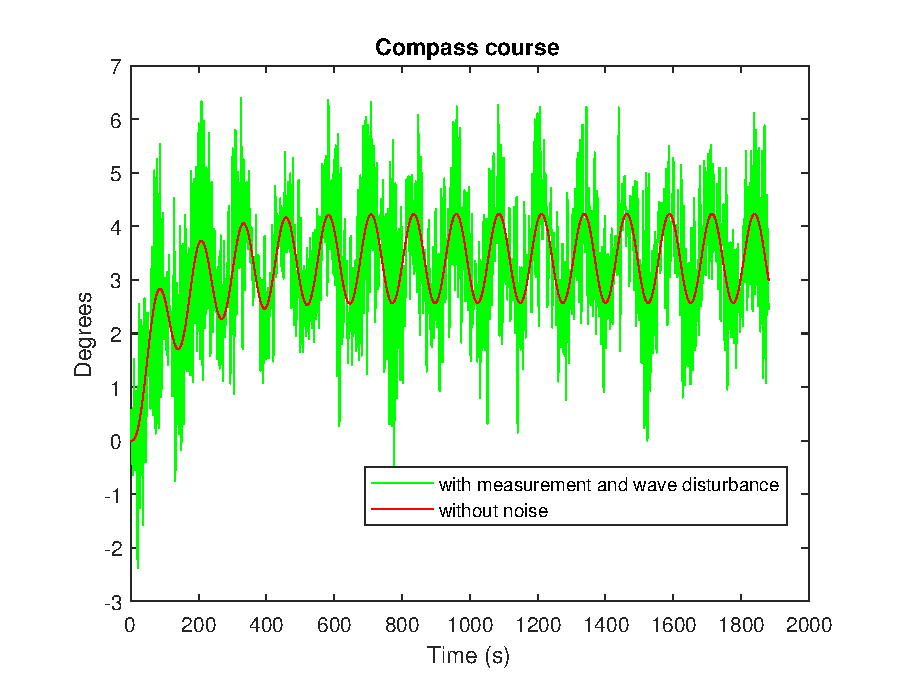
\includegraphics[width=0.5\linewidth]{Part1_pics/p1c_omega2_comp.eps}
    \caption{Compass comparison with $\omega_2$ and added noise}
    \label{fig:p1c2}
\end{figure}

\subsection{Step response}
Oppg: Apply a step input of 1 degree to the rudder at t = 0 and compare the step response of the model with the response of the ship. Is the model a good approximation?
\bigskip

SIMULINK modeller og plots
\bigskip

Modellen følger skipet ganske bra de første 0.5 sek og deretter blir det større avvik fra modell og skip. Der modellen får en lavere verdi enn skipet. 